\chapter{数据、接口与部署设计}

\section{知识数据设计}

知识构建脚本读取\textbf{官方DOCX资料}，解析结构化景点和导览章节，再生成景点实体、知识分块与来源元数据。每个分块保留文档名、章节、景点标识、正文和关键词，使检索结果能够形成\textbf{可读引用}。当前产物包含\textbf{22个景点实体和44个知识分块}，其中主景区与子景区通过\filepath{scenic_area}字段区分。

\begin{table}[H]
  \centering
  \caption{知识库核心数据结构表}\label{tab:knowledge-model}
  \begin{tabularx}{\textwidth}{p{0.18\textwidth}p{0.23\textwidth}X p{0.16\textwidth}}
    \toprule
    对象 & 关键字段 & 设计作用 & 当前规模 \\
    \midrule
    景点实体 & id、name、aliases、culture、highlights、open\_info & 精确识别景点、别名、开放信息与文化特征 & 22条 \\
    知识分块 & documentId、title、content、keywords、scenicSpotId & 作为检索最小证据单元，保留来源关系 & 44条 \\
    检索用例 & query、expectedTitle、expectedSpot、expectedTerms & 验证Top-1、Top-3和关键词召回 & 20条 \\
    问答用例 & question、scenario、label、terms、spot & 验证答案场景、标签、引用与实体 & 50条 \\
    上传文档 & fileName、fileType、status、chunkCount & 支持后台文档管理与知识重建状态追踪 & 数据库持久化 \\
    \bottomrule
  \end{tabularx}
\end{table}

\begin{figure}[H]
  \centering
  \IfFileExists{figures/knowledge-console.png}{%
    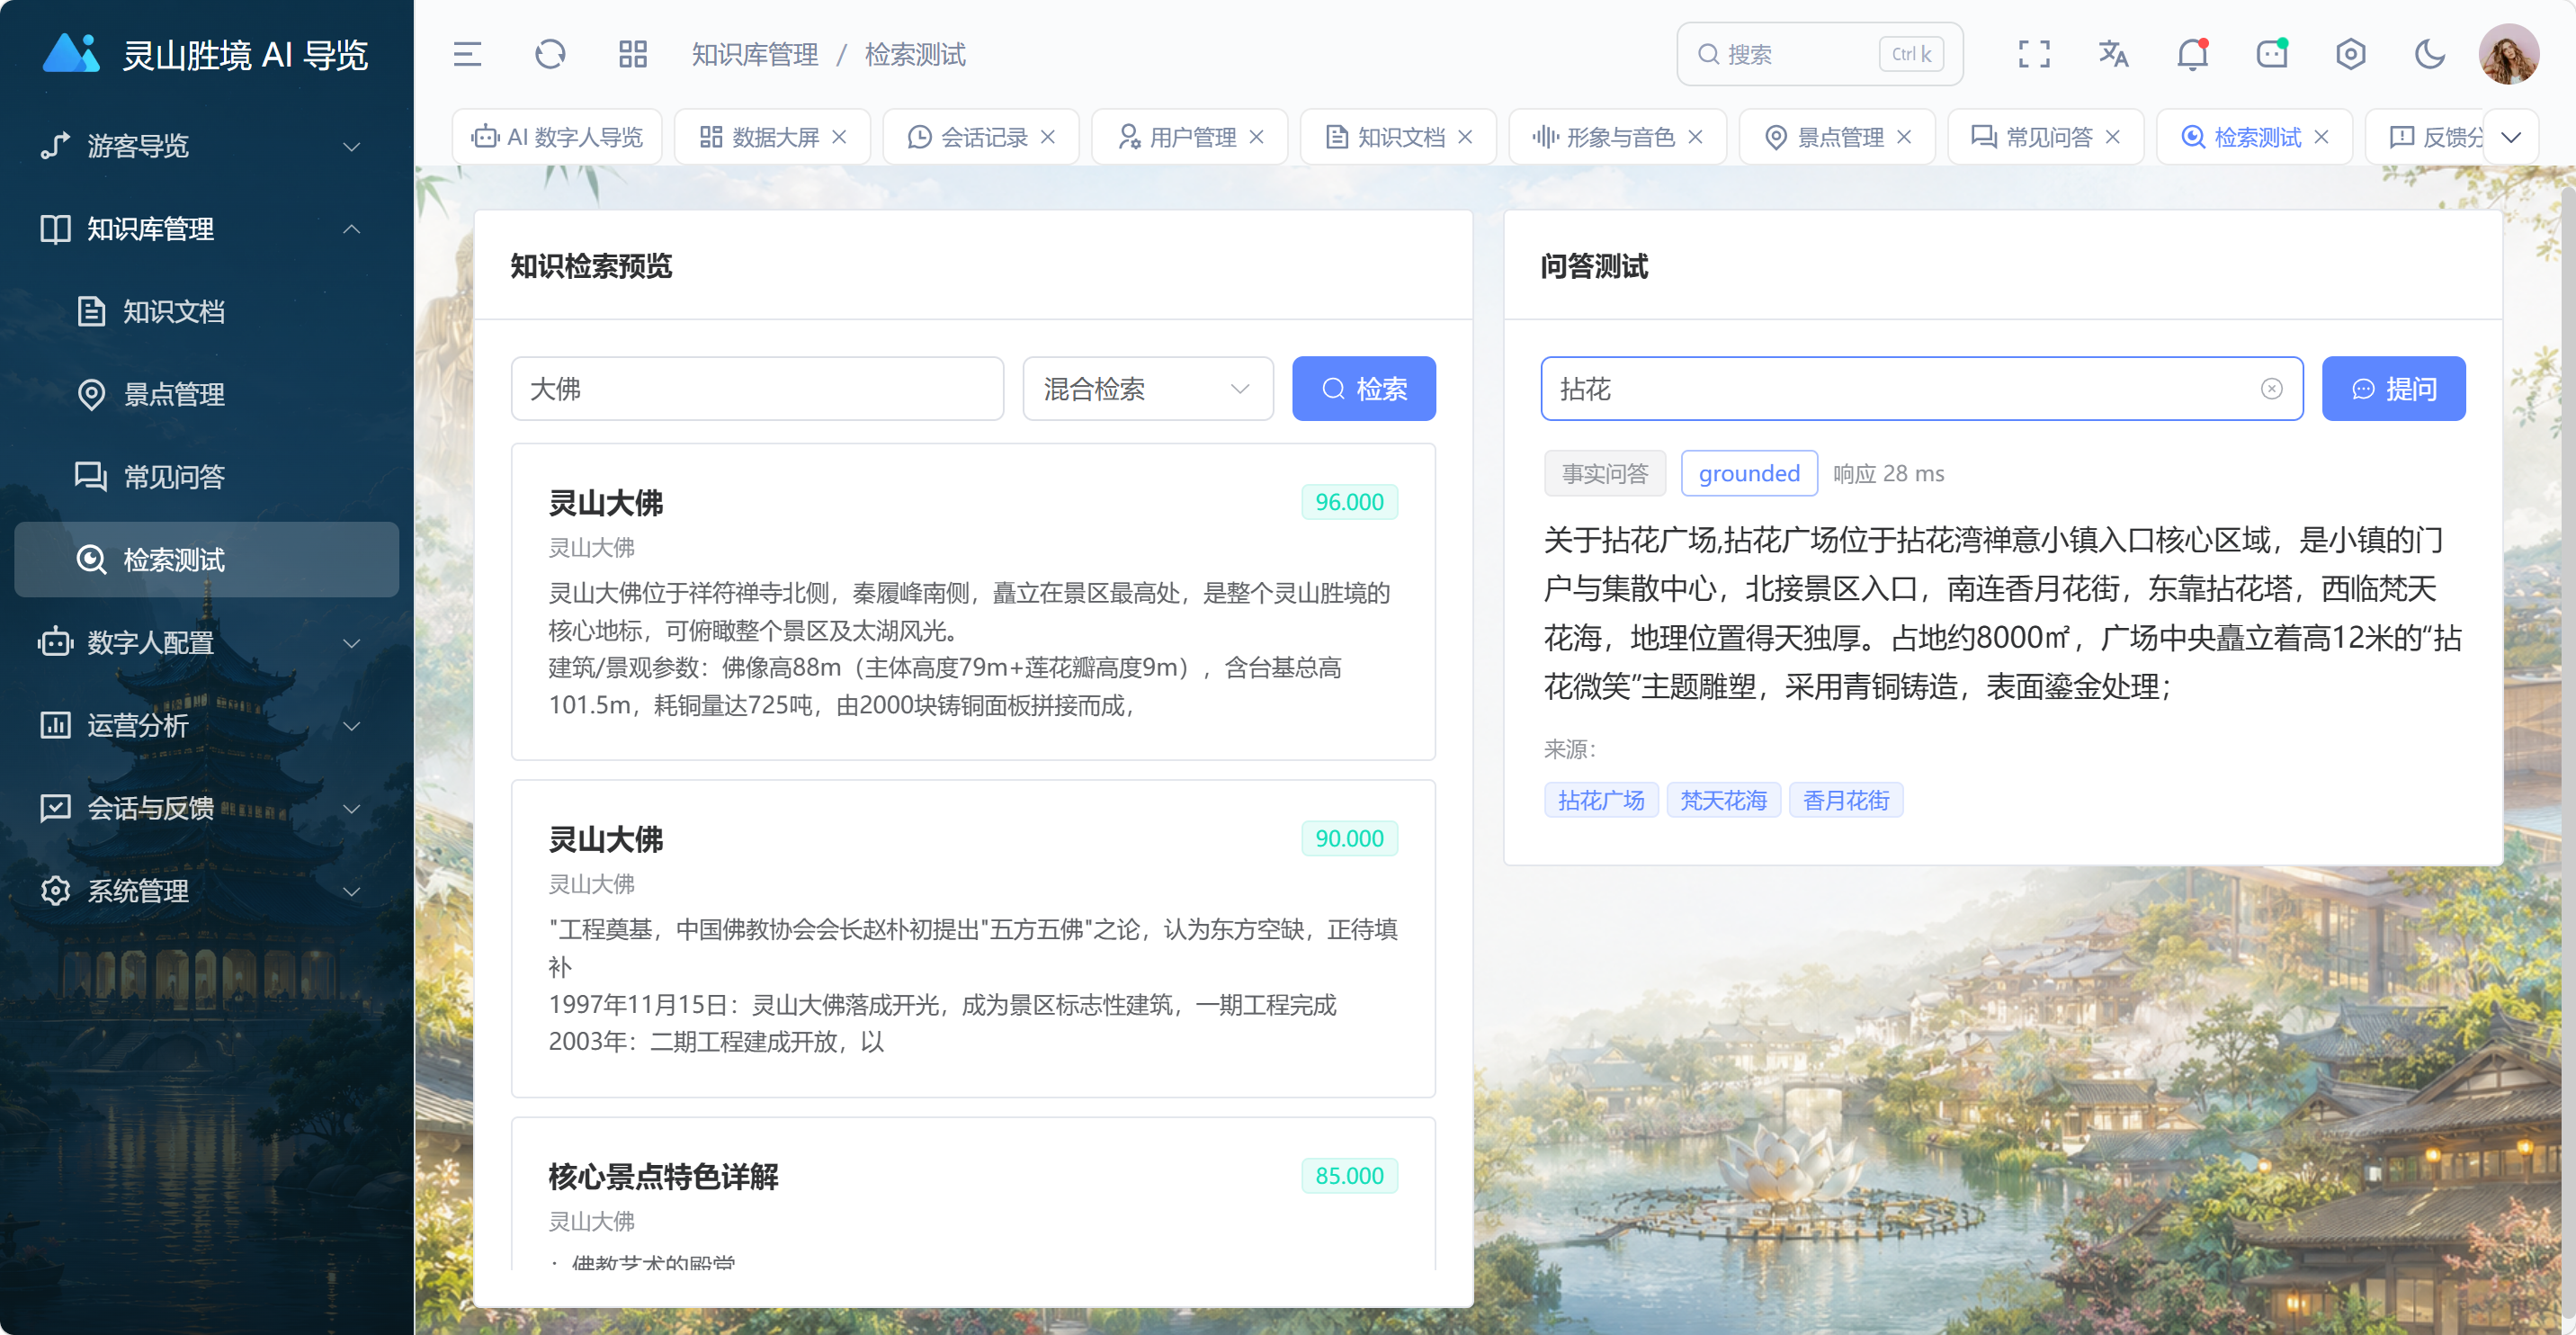
\includegraphics[width=0.95\textwidth]{figures/knowledge-console.png}%
  }{%
    \begin{tikzpicture}[x=1cm,y=1cm]
      \draw[rounded corners=5pt,very thick,guideTeal,fill=guideTealLight] (0,0) rectangle (14.2,6.6);
      \fill[guideTeal] (0,5.95) rectangle (14.2,6.6);
      \node[anchor=west,text=white,font=\bfseries] at (0.35,6.27) {知识库管理页面截图占位};
      \draw[rounded corners=3pt,fill=white,draw=guideTeal] (0.45,4.55) rectangle (4.20,5.55);
      \node at (2.33,5.05) {文档上传与状态};
      \draw[rounded corners=3pt,fill=white,draw=guideTeal] (4.45,4.55) rectangle (8.20,5.55);
      \node at (6.33,5.05) {知识分块统计与重建};
      \draw[rounded corners=3pt,fill=guideGoldLight,draw=guideGold] (8.45,4.55) rectangle (13.75,5.55);
      \node at (11.10,5.05) {混合检索测试与命中分数};
      \draw[rounded corners=3pt,fill=white,draw=guideTeal] (0.45,0.55) rectangle (8.20,4.20);
      \node[font=\bfseries] at (4.33,3.85) {文档与景点维护表};
      \foreach \y in {1.10,1.65,2.20,2.75,3.30}{\draw[guideGray!70] (0.85,\y) -- (7.80,\y);}
      \foreach \x in {2.15,4.15,6.15}{\draw[guideGray!50] (\x,0.90) -- (\x,3.55);}
      \draw[rounded corners=3pt,fill=white,draw=guideGold] (8.45,0.55) rectangle (13.75,4.20);
      \node[font=\bfseries] at (11.10,3.85) {检索结果预览};
      \draw[guideGold] (8.90,2.85) rectangle (13.30,3.40);
      \draw[guideGold] (8.90,1.95) rectangle (13.30,2.55);
      \draw[guideGold] (8.90,1.05) rectangle (13.30,1.65);
    \end{tikzpicture}%
  }
  \caption{知识库文档与检索管理页面图}\label{fig:knowledge-ui}
\end{figure}

\newpage
\section{业务数据与持久化}

SQLite实际建表覆盖管理员、游客会话、消息、反馈、景点、数字人配置、FAQ、知识文档、游客行为、路线选择和消息标注等业务对象。\textbf{事务型数据进入SQLite}；可从官方材料重建的\textbf{知识分块继续保存在JSON中}，从而避免将大段文本与高频会话写入混在同一数据路径。

\begin{table}[H]
  \centering
  \caption{SQLite业务表职责划分表}\label{tab:database}
  \begin{tabularx}{\textwidth}{p{0.25\textwidth}X p{0.25\textwidth}}
    \toprule
    表组 & 主要数据 & 生命周期与用途 \\
    \midrule
    admin\_users & 管理员、运营人员、角色和密码摘要 & 长期保存；管理端鉴权与权限控制 \\
    visitor\_sessions、messages、feedback & 会话、消息标签、时延、评分和文本反馈 & 持续积累；历史恢复与服务质量分析 \\
    scenic\_spots、admin\_faqs、knowledge\_documents & 景点覆盖、固定问答、上传文档状态 & 运营维护；影响问答和知识重建 \\
    digital\_human\_configs & 引擎、讯飞形象ID、Live2D模型ID、VCN、欢迎语、语速、情绪和服务状态 & 唯一启用配置下发游客端；支持云端与本地模型人工切换 \\
    tourist\_behavior、route\_selections & 线下消费行为和游客路线选择 & 运营分析；形成画像和路线偏好 \\
    message\_annotations & 正确、错误、需补知识等人工标注 & 质量闭环；生成知识补充草稿 \\
    \bottomrule
  \end{tabularx}
\end{table}

\section{接口规范}

后端以\filepath{/api}为\textbf{统一前缀}，OpenAPI合同记录\textbf{40条路径、45项操作}。成功响应采用\texttt{\{success,data,meta\}}，失败响应采用\texttt{\{success,error\}}；管理接口要求Bearer Token，游客接口使用匿名会话标识。请求日志记录方法、路径、状态码和耗时；长回答另提供SSE流式接口。接口命名遵循资源化路径，并将\textbf{检索证据、标签和阶段耗时}作为一等输出，便于前端展示与后台追踪。

\newpage
\section{部署拓扑}

生产模式下先构建Web产物，再由\textbf{Node.js同源提供静态资源、SPA回退和API}，减少跨域与多服务配置。数据库、知识库和Live2D模型位于本机数据或静态资源目录，讯飞数字人、大模型和语音能力通过HTTPS/WSS访问；讯飞形象流不可用时可由管理员启用\textbf{本地Live2D配置}，无密钥或其他云服务异常时，\filepath{DEMO_MODE}进入\textbf{本地确定性链路}。部署关系如图\ref{fig:deployment}所示。

\begin{figure}[H]
  \centering
  
\includegraphics[width=0.98\textwidth]{deployment-topology.pdf}
  \caption{系统单机同源与云能力部署拓扑图}\label{fig:deployment}
\end{figure}

\textbf{配置项按职责拆分}：后端保存端口、模型提供者、数据库路径和演示模式；前端保存讯飞应用凭证、服务地址、形象与音色默认值，并随构建产物部署Live2D Cubism运行时及Haru、Hiyori、Kei、Hibiki四套模型。运行配置中的\filepath{engine}、\filepath{avatar_id}、\filepath{model_id}和\filepath{vcn}\textbf{决定游客端实际加载路径}。\textbf{密钥文件不纳入版本控制}，部署前使用\filepath{npm run env:check}检查Node版本、数据文件、目录、端口和云端凭证。
